\documentclass[12pt]{article}
\usepackage[latin1]{inputenc}
\usepackage[english]{babel}
\usepackage{amsmath}
\usepackage{amssymb}
%\usepackage{dsfont}
\usepackage{theorem}
\usepackage{graphicx}
\usepackage{hyperref}
\usepackage{lscape}
\usepackage{enumerate}
\usepackage{verbatim}
\usepackage{float}
\usepackage{fancyhdr}
%\usepackage{bigints}
\pagestyle{fancy}

\newtheorem{theorem}{Theorem}[section]
\newtheorem{lemma}[theorem]{Lemma}
\newtheorem{proposition}[theorem]{Proposition}
\newtheorem{corollary}[theorem]{Corollary}

\newenvironment{proof}[1][Proof:]{\begin{trivlist}
\item[\hskip \labelsep {\bfseries #1}]}{\end{trivlist}}
\newenvironment{definition}[1][Definition:]{\begin{trivlist}
\item[\hskip \labelsep {\bfseries #1}]}{\end{trivlist}}
\newenvironment{example}[1][Example:]{\begin{trivlist}
\item[\hskip \labelsep {\bfseries #1}]}{\end{trivlist}}
\newenvironment{remark}[1][Remark:]{\begin{trivlist}
\item[\hskip \labelsep {\bfseries #1}]}{\end{trivlist}}

\newcommand{\qed}{\nobreak \ifvmode \relax \else
      \ifdim\lastskip<1.5em \hskip-\lastskip
      \hskip1.5em plus0em minus0.5em \fi \nobreak
      \vrule height0.75em width0.5em depth0.25em\fi}

\newcommand*{\QEDA}{\hfill\ensuremath{\blacksquare}}
\newcommand*{\QEDB}{\hfill\ensuremath{\square}}

\newcommand{\dif}{\mbox{d}}


%---------------------------------
%\topmargin -.5 in
%\textheight 22 cm
%\textwidth 16 cm
%\oddsidemargin 0 cm
%\evensidemargin 0 cm
%---------------------------------


\title{Growing Degree Days in Canada - Data Project}
\author{A. Naveen, C. Chagas, A. Iyer, O. Abramov, E. Kielley, R. Brecht}
\date{\today}

\begin{document}

\maketitle
\vspace{5pt}
\tableofcontents
\vspace{35pt}

\section{Motivation}
We want to use Python and Bash scripts to analyse growing degree days (GDD) for 
three different cities in Canada. Growing degree days are used to predict when a 
flower or plant will bloom. 
\\ Plants require energy to grow and develop, and some of this energy is in the 
form of heat. The heat required is expressed as degrees of temperature. 
Temperature regulates many of the physical and chemical processes within a 
plant, which in turn control the rate of growth and development toward maturity. 
\\The amount of heat accumulated during the day, as obtained by subtracting the
 plant's base temperature from the mean temperature for the day, is termed the
 degree-day accumulation.
\\The growing degree days helps to identify the limits of geographical areas 
suitable for production of various crops, particularly corn, and to evaluate 
areas agriculturally suitable for new or non-native plants. Other applications
of degree-days include the prediction of bloom date, tree fruit development, and
insect activity related to agriculture and forestry.


\pagebreak


\subsection{Files and Scripts}
\begin{description}
\item[calc\_gdd.py]
\item Input: min\_temp\_vect, max\_temp\_vect, tbase, tupper
\item Output: (res\_day, res)
\item Calculates the gdd. %TODO


\item[gdd.py]
\item Input: tbase, tupper, input\_folder (optional)
\item Output: year\_cityName\_tbase\_tupper\_gdd.csv
\item Searches for files that ends with \emph{temp.csv}. We expect, that these
files have the columns: Date/Time, Min Temp(${}^\circ$C), Max Temp(${}^\circ$C).

Then these columns of each file will be copied into a new csv file with the name
\emph{year\_cityName\_tbase\_tupper\_gdd.csv}, where cityName is extracted of the
current file name. That file will be saved in the folder \emph{Output}.
After that, a column called GDD will be added. 
The value of
cell $n$ is calculated with the formula:
$$
\sum_{i=1}^n \big( \tfrac{\text{tmax}_i+\text{tmin}_i}{2}-\text{tbase}\big)
$$
If $\text{tmax}_i$ or $\text{tmax}_i$ is bigger than tupper it is set to tupper,
 also if $\text{tmin}_i$ or $\text{tmax}_i$ 
is  smaller than tbase then it is set to tbase.
\\The base temperature,Tbase, is that temperature below which plant growth is zero.
 GDUs are accumulated by adding each day's GDs contribution as the season progresses.
\\ The maximum temperature,Tupp, is usually capped at 30 ${}^\circ$C because most plants and 
insects do not grow any faster above that temperature.
%\item[gdd.sh]
%\item Input: temperatures.csv, tbase, tupper
%\item Output:
%\item What it does... maybe adding code

\item[create\_plots.py]
\item Output: CumulativeGDD.png, CompareMaxMinTemp.png, AnalyzeTbase.png, gddMapPlotNL.png
\item The script consists of functions:
\begin{itemize}
\item max\_min\_plot(names) $\to$ CompareMaxMinTemp.png \\
Shows the maximum and minimum temperatures for Montral, Ottawa and Victoria during the year of 2015 (Task 1.2).
\item gdd\_plot(names)  $\to$ CumulativeGDD.png \\
Shows the cumulative GDD for each city aforementioned in the year of 2015 (Task 1.4).
\item map\_plot\_nl\_gdd()  $\to$  gddMapPlotNL.png \\
Creates a colored map showing how the growing degree days affect Canada (Task 2.2).
\item analyze\_tbase()  $\to$ Analyze\_Tbase.png \\
Shows the accumulated GDD when the tbase is different from the default (Task 2.3).
\item bokeh\_plot\_temp(fname)  
\item bokeh\_plot\_gdd(fname) \\
Shows the interactive plots in html format for selected cities (Task 2.4).
\end{itemize} 
\item Searches for files ending with \emph{gdd.csv}. 
In each file, it reads the max and min temperatures columns and the cumulative 
GDD to create the subplots and/or maps required to complete the tasks. 
Finally saves the created figures as PNG-files in the \emph{Plot} folder.

\end{description}
\subsection{Process flow}
The following diagramm shows the dependencies and execution steps of the scripts
we are running.
\\~\\
By executing the \emph{Makefile}, we create a folder called \emph{Output} and run
the python script \emph{gdd.py} with the arguments tbase=10, tupper=30 and the path
 \emph{./Input/}. This produces 3 csv files, because we have 3 files of the 
format \emph{year\_cityName\_.csv} in the folder \emph{Input}.
Next the script \emph{create\_plots.py} is called by Makefile and produces 2 PNG-
files. Finally Makefile creates the file \emph{report.pdf} by compiling the 
\emph{report.tex} file.

	\begin{figure}[!htbp]
		\centering
		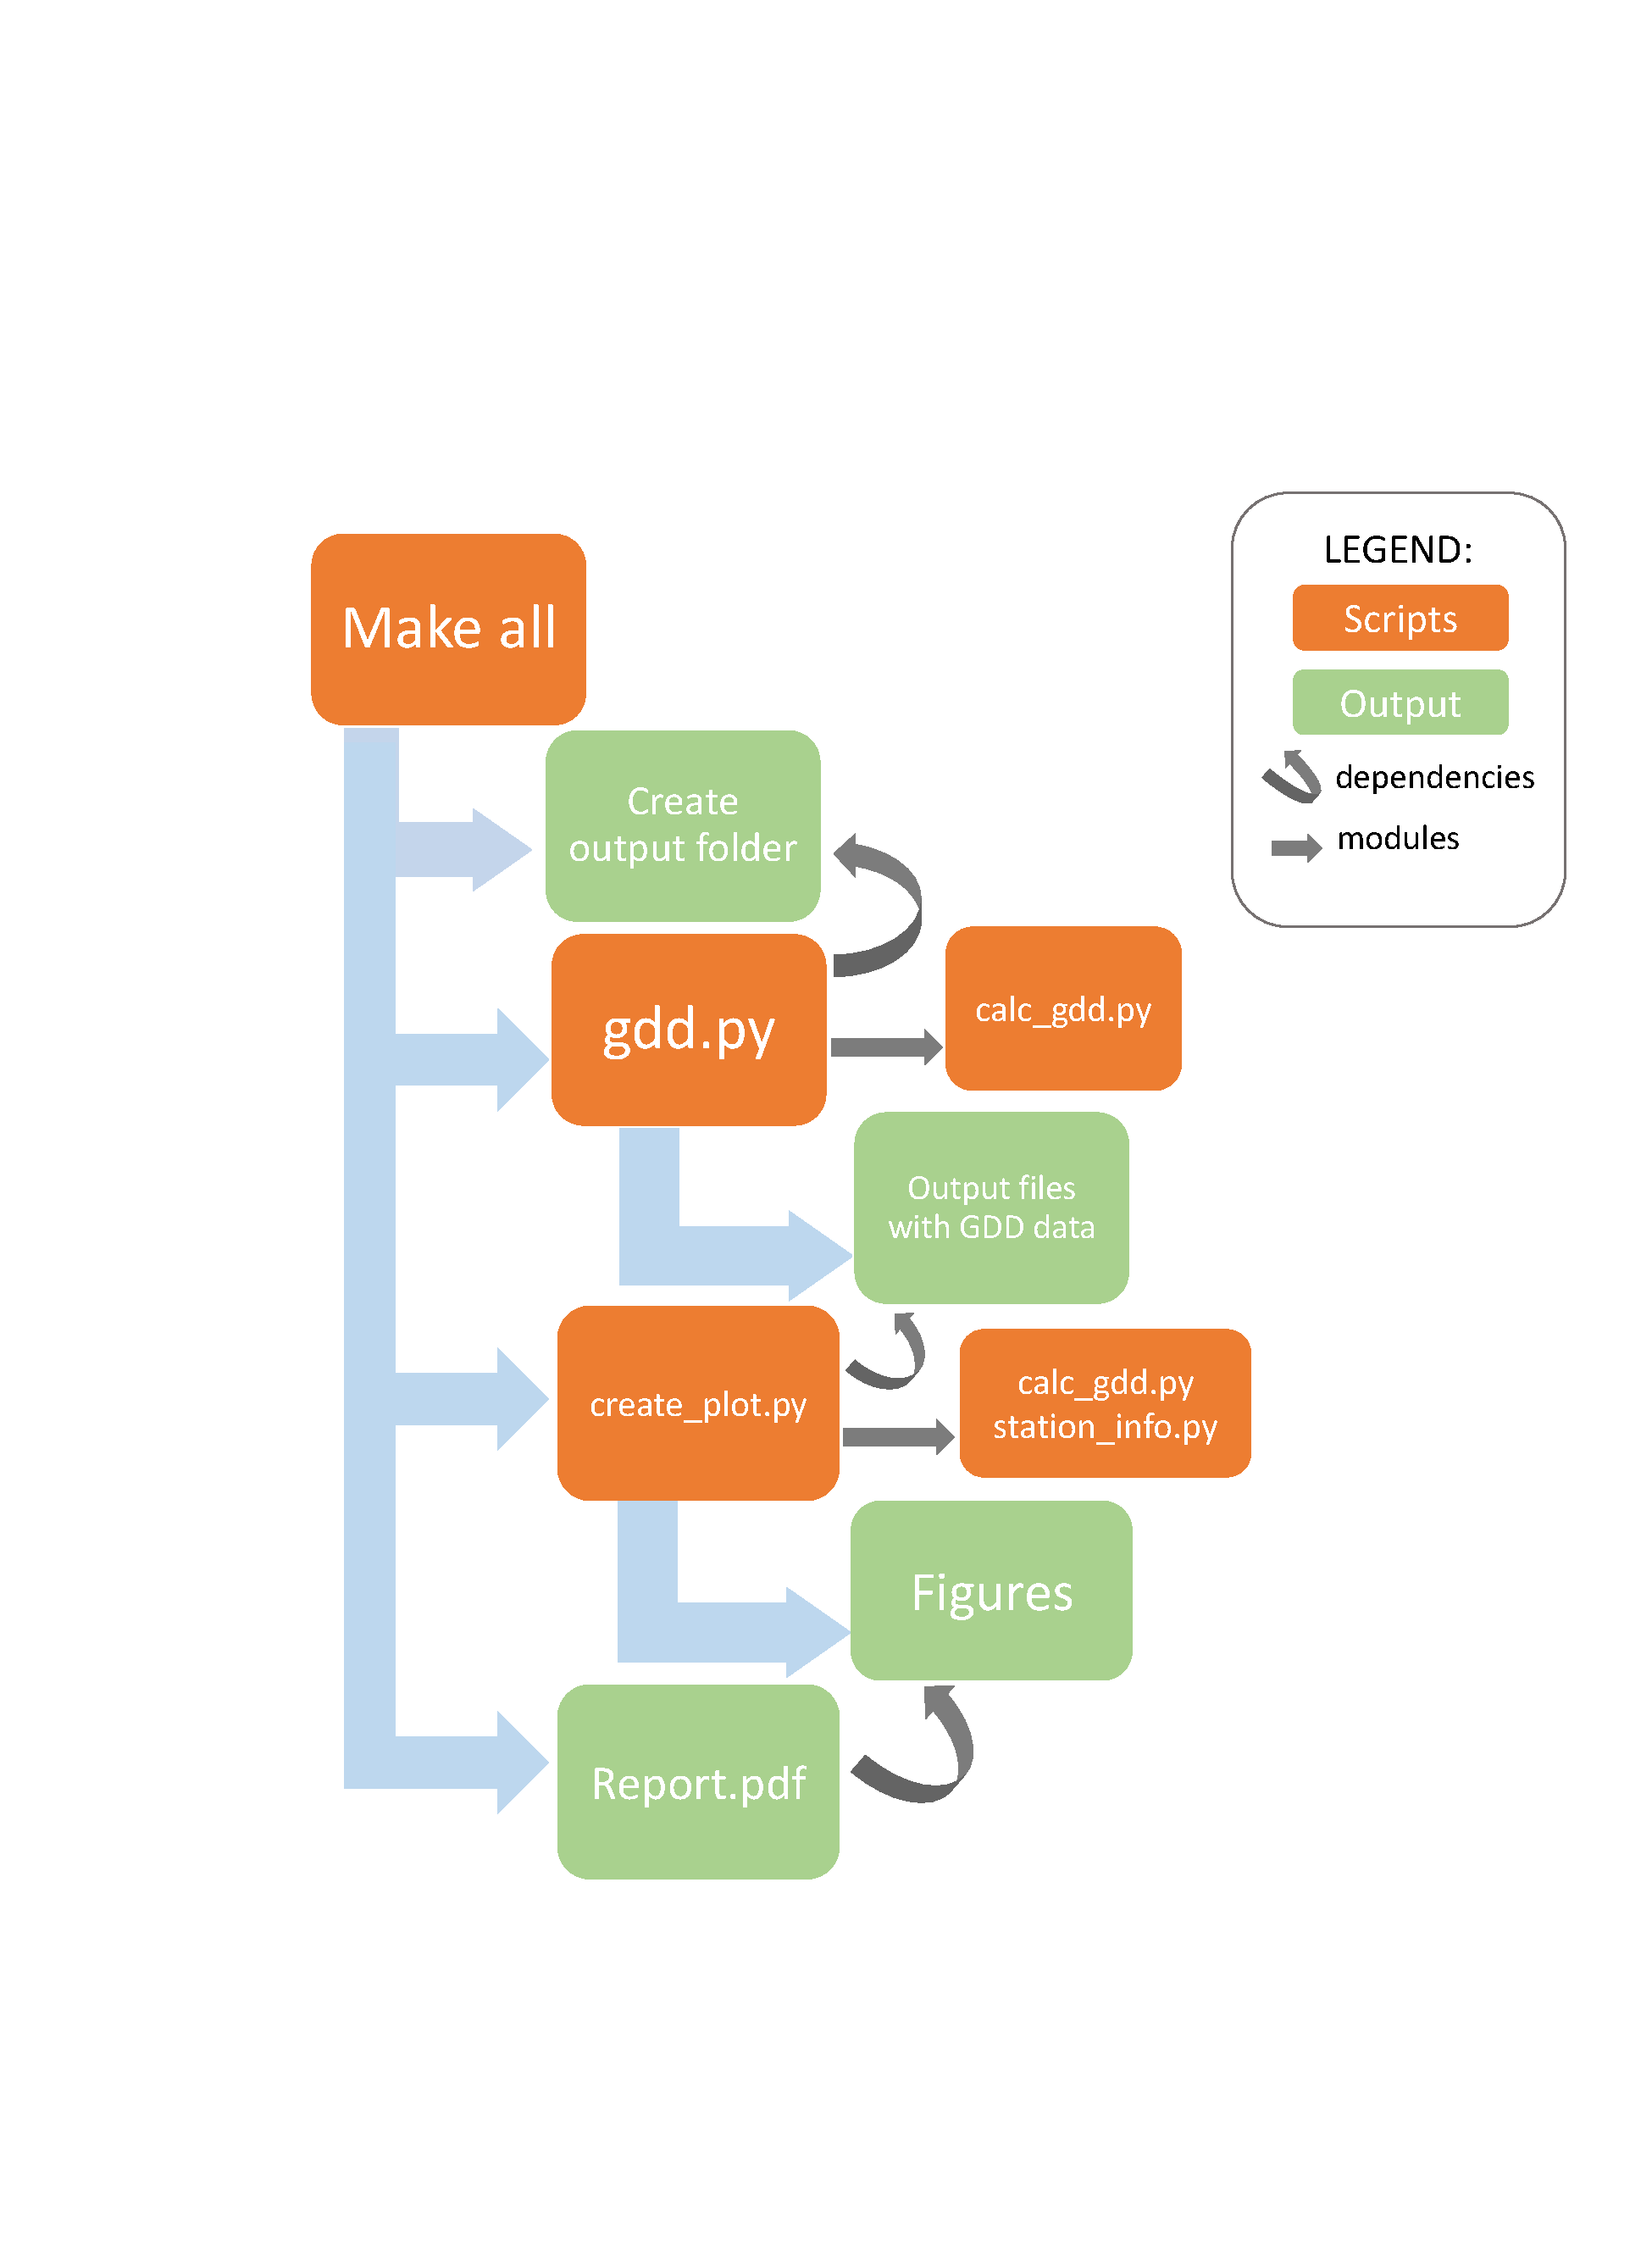
\includegraphics[width=0.9\textwidth]{./Report/diagram_workflow.pdf} 
		\caption{\scriptsize Shows the process flow of our scirpts.}\label{flowplot}		  
	\end{figure}


\pagebreak

\subsection{Results}
	\begin{figure}[!htbp]
		\centering
		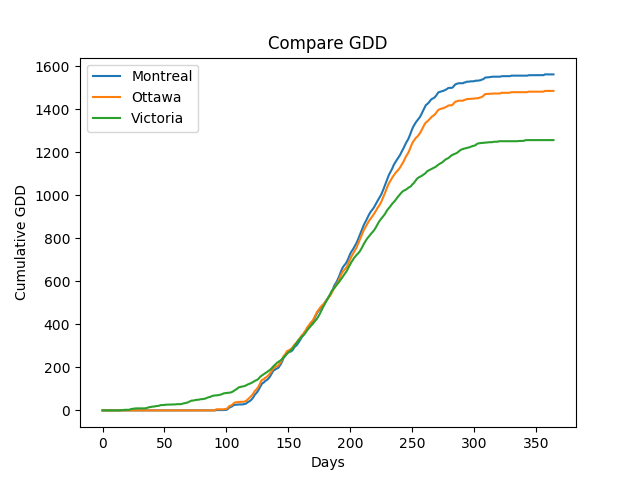
\includegraphics[width=0.9\textwidth]{./Output/CumulativeGDD.png} 
		\caption{\scriptsize Shows the accumulated GDD vs time for three selected cities.}\label{GDDplot}		  
	\end{figure}

	\begin{figure}[!htbp]
		\centering
		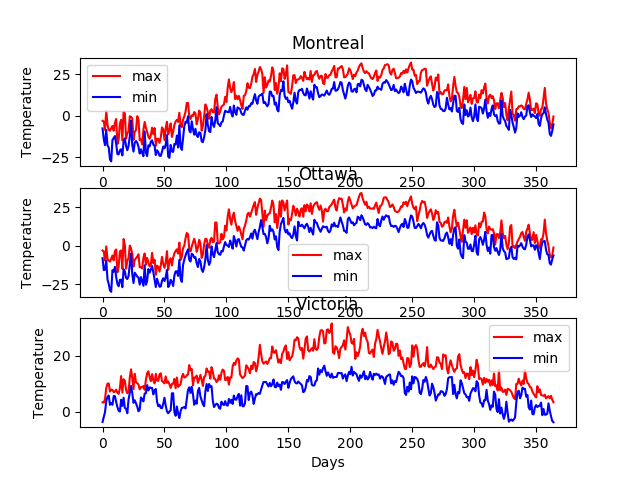
\includegraphics[width=0.9\textwidth]{./Output/CompareMaxMinTemp.png} 
		\caption{\scriptsize Shows the min and max temperature for three selected cities.}\label{MinMaxplot}		  
	\end{figure}

	\begin{figure}[!htbp]
		\centering
		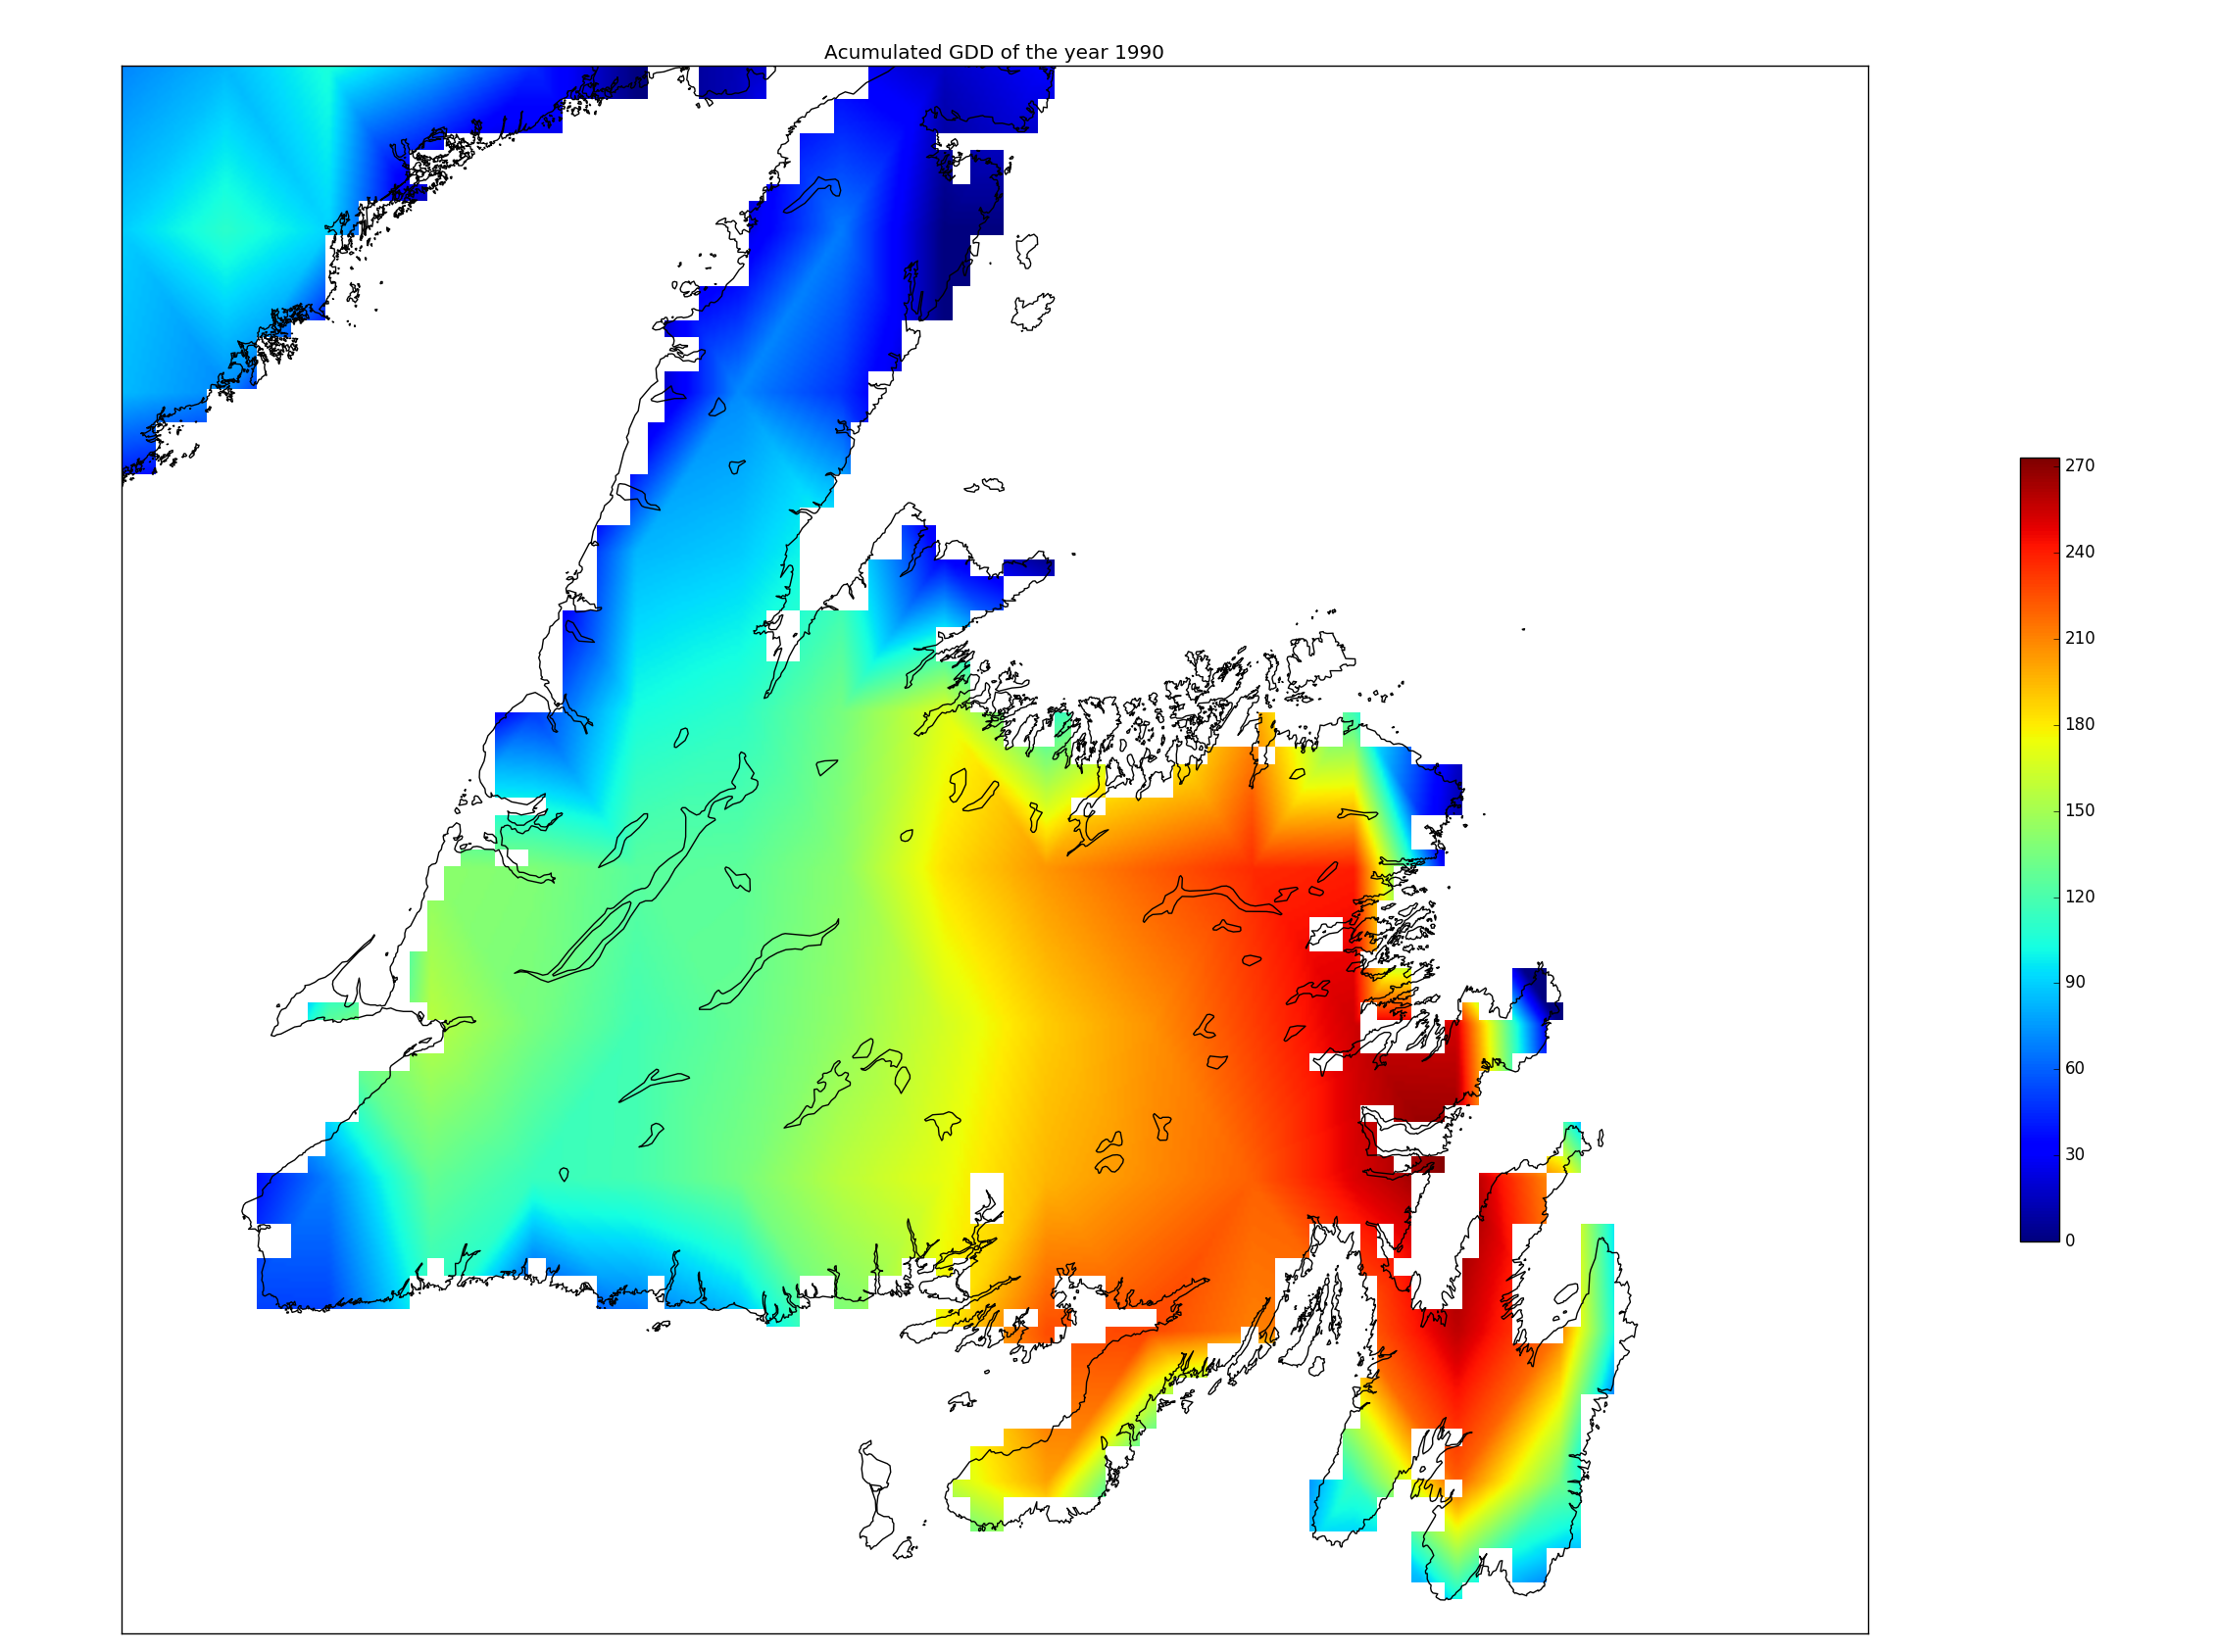
\includegraphics[width=0.9\textwidth]{./Output/gddMapPlotNL.png} 
		\caption{\scriptsize Shows an interpolated map plot of gdd data.}\label{gddMapNl}		  
	\end{figure}

	\begin{figure}[!htbp]
		\centering
		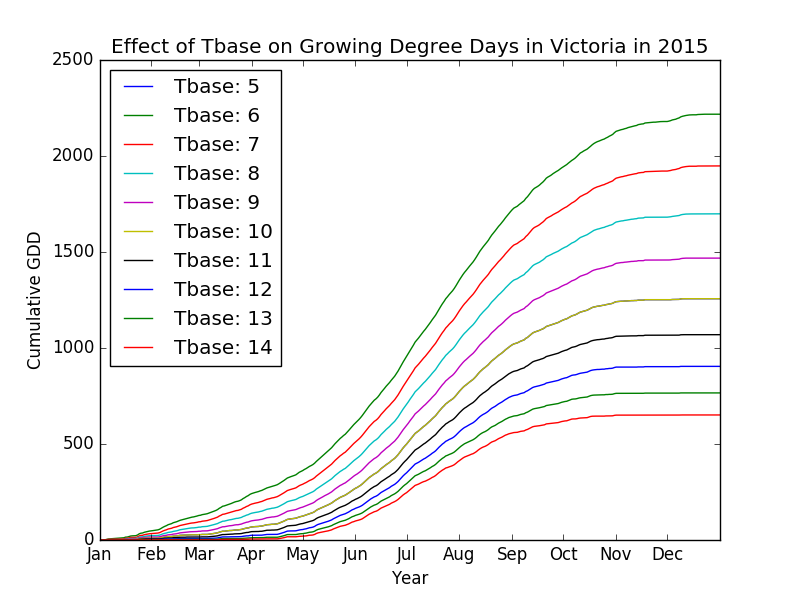
\includegraphics[width=0.9\textwidth]{./Output/AnalyzeTbase.png} 
		\caption{\scriptsize Figure shows comparison of different tbase choices.}\label{gddMapNl}		  
	\end{figure}

For example, suppose you plant Red Maple in different areas on May 15th.
The tree has a base temperature of 10${}^\circ$C and requires 27 GDD to reach maturity.
	\begin{figure}[!htbp]
		\centering
		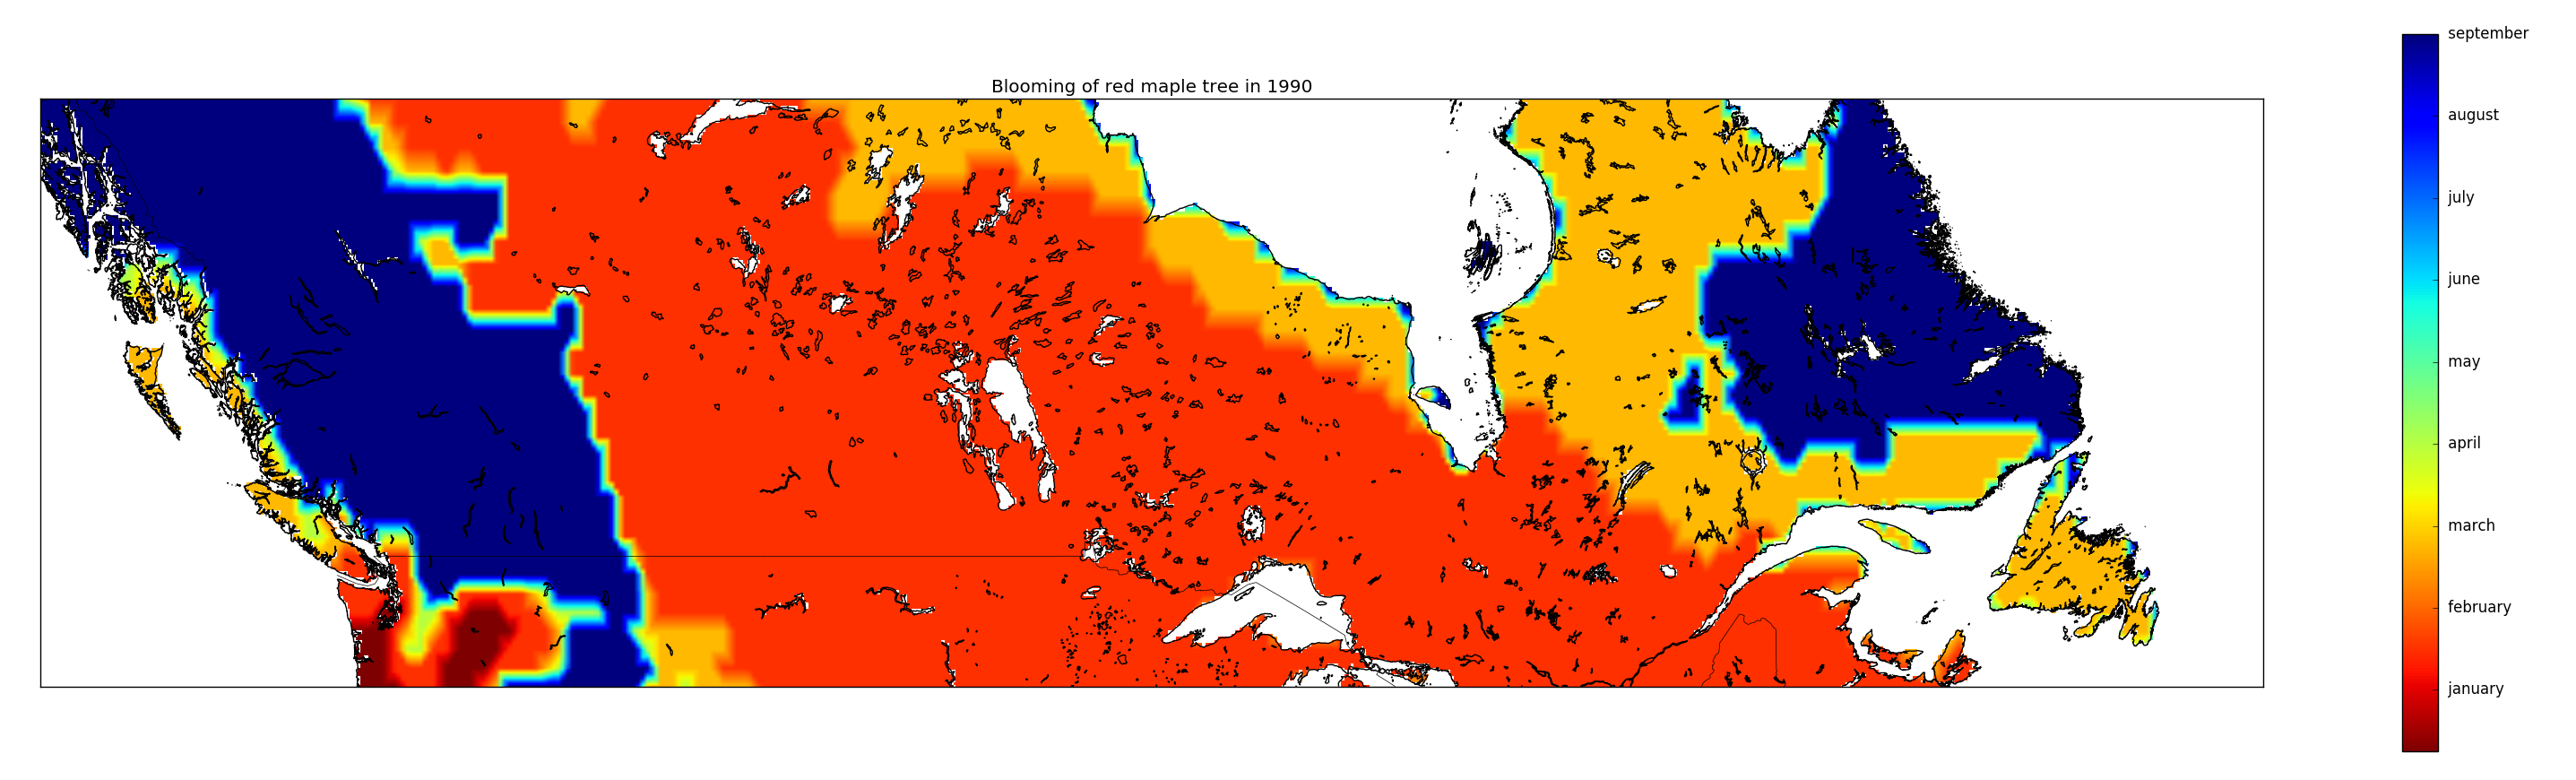
\includegraphics[width=0.9\textwidth]{./Output/CanadaBloomingOfMaple.png} 
		\caption{\scriptsize Figure shows...}\label{gddMapCaMaple}		  
	\end{figure}


\end{document}
